%!TEX root = ../dissertation.tex

\chapter{Background}

\section{Donder's and Listing's laws}
\label{appendix:cha1:listings}

Donders' law states that the orientation of the eye, when looking in a specific direction at infinity, is always the same; in other words, as described by Donders: "with the head erect and looking at infinity, any gaze direction has a unique torsional angle, regardless the path followed by the eye to get there". Thus, the eye has 2 degrees of freedom for pointing.

Moreover, the 3D orientations of the eye can be uniquely described by head-fixed Cartesian coordinate system of single-axis rotations (section \ref{killme}) that bring the eye from the primary position to the current orientation. Described in this way, Listing's law holds that the rotation axis corresponding to all possible eye orientations is confined to the yz-plane, called Listing's plane. The primary position of the eye is an unique position from which any other eye position can be reached through rotation around an axis lying in Listing's plane. This hypothetical rotation axis is defined by a vector, $ \mathbf{r}$, the torsional component perpendicular to the Listing's plane, is zero. 
Figure \ref{sec2:fig:monkey} illustrates that this law is very precise, by showing 3500 different eye orientations made by a head-restrained monkey, where the left image is the frontal view on the rotation axis, representing the gazed points coordinates of the horizontal and vertical components of the axis, and the right-hand plot is a side view, representing the coordinates expressed by the  horizontal and torsional components. A plane is clearly seen around $0 \ degrees$ of torsion with little deviation ($\approx 0.6$ deg).
\begin{figure}[ht]
	\centering
	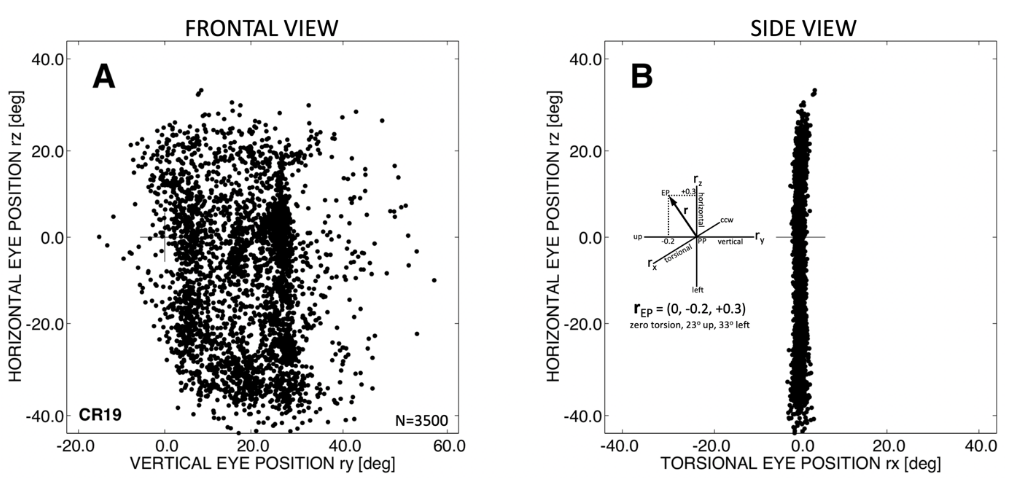
\includegraphics[width=13cm]{images/ll.png}
	\caption[Listing’s law, illustrated for 3500 eye orientations made by a head-restrained monkey]{Listing’s law, illustrated for 3500 eye orientations made by a head-restrained monkey, freely looking around in the laboratory room. Eye fixations are represented by the head-fixed Cartesian components of the 3D rotation axes, expressed in half-radians, and calculated as $angle = 2 \cdot atan(component)$. \cite{donders}}
	\label{sec2:fig:monkey}
\end{figure}
\cite{donders} 

\section{\acrlong{sift}}
\label{appendix:cha1:sift}
The \acrshort{sift} algorithm consists of a local feature detector and local histogram-based descriptor. At first, \acrshort{sift} takes the original image, and generates progressively blurred images through a Gaussian filter as $L (u , v , \sigma ) = G ( u , v, \sigma ) * I ( u , v )$, where $(u, v)$ are the pixel coordinates, $L$ is the blurred image, $I$ is the original image, $G$ is the \gls{gauss}, and finally $\sigma$ is the amount of blur. Then, it re-sizes the original image to half its size, and generates the blurred images again, and repeats. Each new re-sizing of the previous image is scaled by an octave, and each octave can be blurred  several times. This process ensures the scale invariance of potential features.

The set of blurred images obtained, then goes through the Difference of Gaussians (DoG) calculation, to find points of interest, or features, later on. To that end, the images from each octave (scale) are subtracted from each other pairwise, as illustrated in Figure \ref{sec2:fig:DoG}. Mathematically, what happens is obtaining $D ( u , v , \sigma ) = L ( u , v , k \sigma ) - L ( u , v , \sigma )$, where $k$ is a constant multiplicative (scaling) factor and $D$ is the difference.

Then, the search for local maxima/minima on the resulting images takes place. Each point is compared to its eight neighbors in the current image and nine neighbors in the image of one scale above and below, as Figure \ref{sec2:fig:maxima} shows. The points are only selected if they are larger than all of its neighbors or smaller than all of them.

\begin{figure}[ht]
	\begin{minipage}[b]{0.65\linewidth}
		\centering
		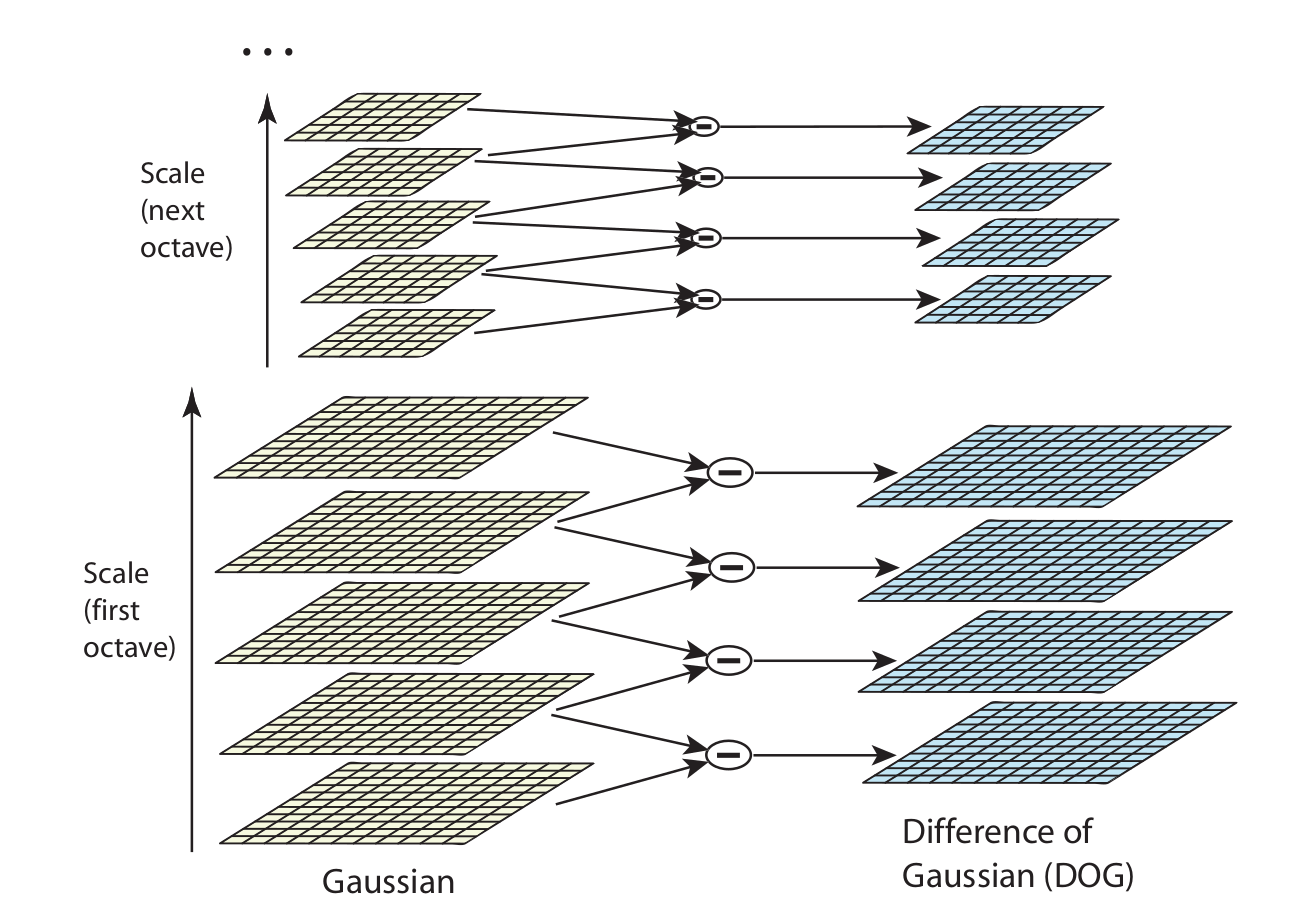
\includegraphics[width=\textwidth]{images/sift1.png}
		\caption[Difference of Gaussians (DoG) by octave]{Difference of Gaussians (DoG) by octave. To find points of interest (features), the Gaussian-blurred images at each scale (octaves) are subtracted pairwise. This process is computationally more efficient than computing the Laplacian of the Gaussians. \cite{sift}}
		\label{sec2:fig:DoG}
	\end{minipage}
	\hspace{0.5cm}
	\begin{minipage}[b]{0.3\linewidth}
		\centering
		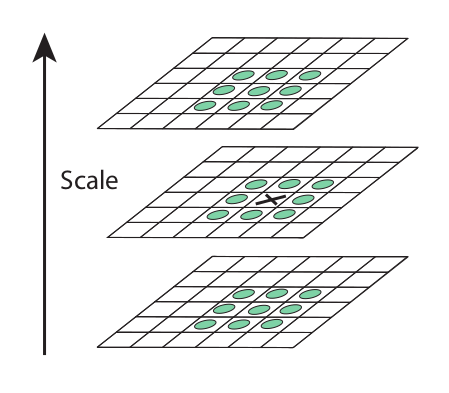
\includegraphics[width=\textwidth]{images/sift2.png}
		\caption[Search for the maxima and minima of the DoG]{Search for the maxima and minima of the DoG. After the DoG, each point is compared with its eight neigbours, and with the 9 corresponding neighbours of the images of the scale above and below. \cite{sift}}
		\label{sec2:fig:maxima}
	\end{minipage}
\end{figure}

The location of this maxima/minima is an approximation since it almost never lies on the exact pixel but somewhere between pixels. Thus, the next step is to search for the feature's exact location by using a Taylor expansion (up to the quadratic terms) of the scale-space function $D(u,v,\sigma)$, shifted from the origin, according to 
\begin{equation}
\label{sec2:eq:subpixel}
D ( \mathbf{x} ) = D + \frac { \partial D ^ { T } } { \partial \mathbf{x} } \mathbf{x}  + \frac { 1 } { 2 } \mathbf{x} ^ { T } \frac { \partial ^ { 2 } D } { \partial \mathbf{x}^ { 2 } } x.
\end{equation}
$D$ and its derivatives are determined at each point by using $\mathbf{x} = (u, v, \sigma)^T$ as an offset.

Apart from removing low-contrast sub-pixels just determined, it's also important to remove edges since the DoG has a strong response to them (delta functions). An unwanted peak in the DoG will have a large gradient perpendicular to the edge but a small gradient along the edge direction, and because of that property it can be easily detected and eliminated. This is accomplished by computing a Hessian matrix on the point.

Finally, to have a rotation invariant feature, it's necessary to create an oriented patch around the point. For each image, $L(u, v)$, at a certain scale, the gradient magnitude, $m_g$ and orientation, $\theta$, are determined as 
\begin{equation}
\label{sec2:eq:descriptor}
\begin{array} { l } { m_g ( u , v ) = \sqrt { ( L ( u + 1 , v ) - L ( u - 1 , v ) ) ^ { 2 } + ( L ( u , v + 1 ) - L ( u , v - 1 ) ) ^ { 2 } } } \\ { \theta ( u , v ) = \tan ^ { - 1 } ( ( L ( u , v + 1 ) - L ( u , v - 1 ) ) / ( L ( u + 1 , v ) - L ( u - 1 , v ) ) ) } \end{array}.
\end{equation}
This information is used to create a histogram of orientations. Peaks on the histogram correspond to dominant directions of local gradients. Local peaks that are within 80\% of the highest peak are used to create more features with that orientation.

\begin{figure}
	\centering
	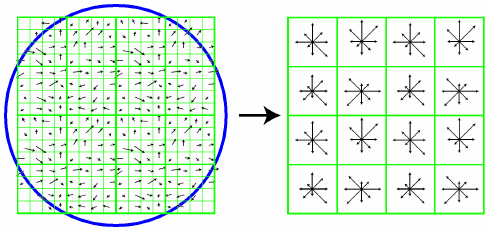
\includegraphics[width=8cm]{images/sift3.png}
	\caption[\acrshort{sift} feature descriptor]{\acrshort{sift} feature descriptor. A window of $16\times16$ squares is centered around the point of interest. The blue circle represents the Gaussain window. In each $4\times4$ sub-region, a histogram of orientations is determined, represented on the image on the right. In total there are $8\times 16 = 128$ values to describe the feature. \cite{sift}}
	\label{sec2:fig:sift3}
\end{figure}
For the descriptor of the feature, a 16$\times$16 window around the point of interest is set. For each $4\times4$ region, the orientations are put into an 8 bin histogram (each bin with a 45 degree range). This can be seen through Figure \ref{sec2:fig:sift3}. The length of each arrow corresponds to the sum of the gradient magnitudes near that direction within the region. Doing this for the 16 regions, there will be 128 values describing the feature.
\cite{sift}

\section{\acrlong{surf}}
\label{appendix:cha1:surf}
\acrshort{surf} starts from an integral image, which is an intermediate representation of the
original image. The entry of an integral image $I_{\Sigma}( \mathbf{x})$ at a location
$\mathbf{x} = (u, v)$ represents the sum of all pixels in the input image $I$ of a rectangular region formed by the point $\mathbf{x}$ and the origin as 
\begin{equation}
\label{sec2:eq:int}
\mathrm { I } _ { \Sigma } ( \mathbf{x} ) = \sum _ { \mathrm { i } = 0 } ^ { \mathrm { i } \leq \mathrm { u } } \sum _ { \mathrm { j } = 0 } ^ { \mathrm { j } \leq \mathrm { v } } \mathrm { I } ( \mathrm { i } , \mathrm { j } ),
\end{equation}
allowing a faster computation with box-type convolution filters. 

The applied box filter is an approximation of Gaussian second-order derivatives. Instead, of having to apply the Gaussian filter iteratively to the output image and to different scales as seen on \acrshort{sift}, this can be done directly with the box filter by up-scaling it and altering its masks in parallel. Figure \ref{sec2:fig:surf} makes a comparison between the Gaussian second-order derivatives, Laplacians $L_{yy}$ and $L_{xy}$, and a box filter applied on a point on the y and xy-direction, $D_{yy}$ and $D_{xy}$.

\begin{figure}[ht]
	\begin{minipage}[b]{0.65\linewidth}
		\centering
		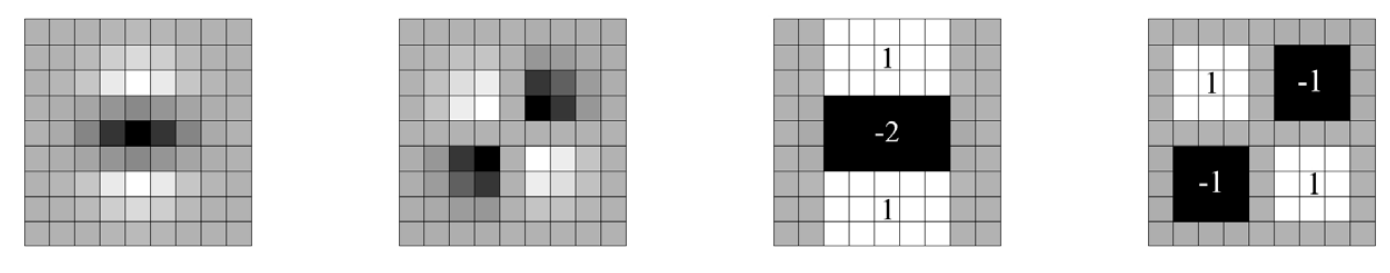
\includegraphics[width=\textwidth]{images/surf.png}
		\caption[Comparison between Gaussian second order derivatives and box filter]{Comparison between Gaussian second order derivatives (from the left, the first image in y-direction - $L_{yy}$ - and second image in xy-direction - $L_{xy}$) and the corresponding images (from the left, the third image in y-direction - $D_{yy}$ - and fourth image in xy-direction - $D_{xy}$) using a box filter. \cite{surf}}
		\label{sec2:fig:surf}
	\end{minipage}
	\hspace{0.5cm}
	\begin{minipage}[b]{0.3\linewidth}
		\centering
		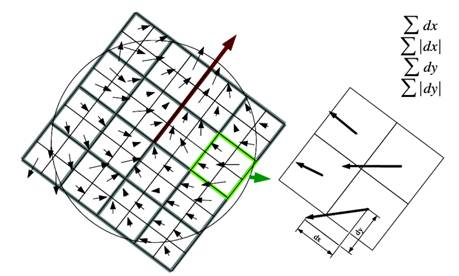
\includegraphics[width=\textwidth]{images/surf2.jpg}
		\caption[\acrshort{surf} feature descriptor]{\acrshort{surf} feature descriptor. The sampling window is rotated towards the dominant orientation. The vector $\left( \sum d _ { x } , \sum d _ { y } , \sum _ { x } \left| d _ { x } \right| , \sum \left| d _ { y } \right| \right)$ is generated per each region through the Haar-wavelet responses in x and y direction. \cite{surf}}
		\label{sec2:fig:surff}
	\end{minipage}
\end{figure}

The Hessian matrix at point $\mathbf{x}$ and scale $\sigma$ is defined as
\begin{equation}
\label{sec2:eq:hessian}
\mathcal { H } ( \mathbf{x} , \sigma ) = \left[ \begin{array} { l l } { L _ { x x } ( \mathbf{x} , \sigma ) } & { L _ { x y } ( \mathbf{x} , \sigma ) } \\ { L _ { x y } ( \mathbf{x} , \sigma ) } & { L _ { y y } ( \mathbf{x} , \sigma ) } \end{array} \right],
\end{equation}
where $L_{xx}(\mathbf{x}, \sigma)$ is the convolution of the Gaussian second-order derivative $\frac { \partial ^ { 2 } } { \partial \mathbf{x} ^ { 2 } } g ( \sigma )$ with the image $I$ at point $\mathbf{x}$, and similarly for $L_{xy}(\mathbf{x}, \sigma)$ and $L_{yy}(\mathbf{x}, \sigma)$, which are weighted on the calculation of the determinant by $w = \frac { \left| L _ { x y } ( 1.2 ) \right| _ { F } \left| D _ { y y } ( 9 ) \right| _ { F } } { \left| L _ { y y } ( 1.2 ) \right| _ { F } \left| D _ { x y } ( 9 ) \right| _ { F } } \approx 0.9$.
The determinant is then defined as 
\begin{equation}
\label{sec2:eq:det}
\operatorname { det } \left( \mathcal { H } _ { a p p r o x } \right) = D _ { x x } D _ { y y } - \left( w D _ { x y } \right) ^ { 2 },
\end{equation}
and is used to find the local change around a point. Points where the determinant is maximal are chosen as features. 

\acrshort{surf}'s feature descriptor was designed to be scale and rotation invariant. The descriptor is sampled over a window that is proportional to the image scale, so that when a scaled version of the feature in another image is found, the descriptor will be sampled relatively, satisfying the scale-invariance requirement.

To obtain rotation invariance, the sampling window is rotated towards the dominant orientation. The window size is 20$s$, where $s$ is the scale at which the point was detected, and is divided into a quadratic grid with 4$\times$4 square sub-regions. For each region, the Haar-wavelet responses are computed in the x and y directions. The descriptor is the sum of the x responses over its four quadrants, sum of the absolute values of the x responses and similarly for y, hence it may be defined as $\left( \sum d _ { x } , \sum d _ { y } , \sum _ { x } \left| d _ { x } \right| , \sum \left| d _ { y } \right| \right)$. Having 4 values per region and 16 regions, yields a total of 64 values to describe the feature. Figure \ref{sec2:fig:surff} helps at visualizing the process.

The dominant orientation, here lightly and carelessly explained, is captured through the calculation of Haar-wavelet responses over a circular region around the point of interest with a radius of 6$s$. Those responses are then summed within a sliding orientation window covering an angle of $\frac{\pi}{3}$. \cite{surf} \cite{compsiftsurf}

\section{Factorization of the essential matrix}
\label{appendix:cha1:epipolar}
To obtain the camera matrix from the essential matrix, the following should be considered.
A $3 \times 3$ matrix is an essential matrix if and only if two of its singular values are equal, and the third is zero. This is easily proven by the decomposition of $E = SR$, where $S$ is a \gls{skews}.
Considering the matrices 
\begin{equation}
\mathrm { W } = \left[ \begin{array} { c c c } { 0 } & { - 1 } & { 0 } \\ { 1 } & { 0 } & { 0 } \\ { 0 } & { 0 } & { 1 } \end{array} \right] \quad \text { and } \quad \mathrm { Z } = \left[ \begin{array} { c c c } { 0 } & { 1 } & { 0 } \\ { - 1 } & { 0 } & { 0 } \\ { 0 } & { 0 } & { 0 } \end{array} \right],
\end{equation}
where $W$ is orthogonal and $Z$ is a \gls{skews}, $S$ may be written as $S = kUZU^T$\footnote{A proof of this is given in Result A4.1 of R. Hartley and A. Zisserman,Multiple View Geometry in Computer Vision \cite{multiview}}, where $U$ is orthogonal and $Z = \operatorname{diag}(1,1,0)W$, up to sign. Thus, $S = U \operatorname { diag } ( 1,1,0 ) WU^T$, up to scale, and 
\begin{equation}
E = SR = U \operatorname { diag } ( 1,1,0 ) \left( WU^T R \right) = U \operatorname { diag } ( 1,1,0 ) V^T,
\end{equation}
proving the initial statement.
Because the singular values have to be equal, the \acrshort{svdd} of $E$ is not unique, in fact 
\begin{equation}
\label{gf}
E = U \operatorname { diag } ( 1,1,0 ) V ^ { T },
\end{equation}
or 
\begin{equation}
E = U \operatorname { diag } ( 1,1,0 ) ( - V ) ^ { T }.
\end{equation} 
Considering (\ref{gf}), because
\begin{equation}
\begin{aligned} 
Z W = \operatorname { diag } ( 1,1,0 ) \\ 
\text{and} \
Z W ^ { T } = - \operatorname { diag } ( 1,1,0 ) ,
\end{aligned}
\end{equation}
$E=SR$ may be decomposed into two forms,
\begin{equation}
\label{ccha}
S = - U Z U ^ { T } , \quad R = U W ^ { T } V ^ { T },
\end{equation}
or
\begin{equation}
\label{ccha2}
S = U Z U ^ { T } , \quad R = U W V ^ { T }.
\end{equation}
(\ref{ccha}) is a rotation matrix and can be proven as such. Since it's orthogonal,
\begin{equation}
R ^ { T } R = \left( U W ^ { T } V ^ { T } \right) ^ { T } U W ^ { T } V ^ { T } = V W U ^ { T } U W ^ { T } V ^ { T } = I,
\end{equation}
and 
\begin{equation}
\operatorname { det } \left( U W ^ { T } V ^ { T } \right) = \operatorname { det } ( U ) \operatorname { det } \left( W ^ { T } \right) \operatorname { det } \left( V ^ { T } \right) = \operatorname { det } ( W ) \operatorname { det } \left( U V ^ { T } \right) = 1,
\end{equation}
which are enough conditions to prove it. Furthermore, $S$ is a \gls{skews} because,
\begin{equation}
- S^ { T } = \left( U Z U ^ { T } \right) ^ { T } = U Z ^ { T } U ^ { T } = - U Z U ^ { T } = S.
\end{equation}
The same applies to (\ref{ccha2}).\footnote{C. Olsson. \href{http://www.maths.lth.se/matematiklth/personal/calle/datorseende13/notes/forelas6.pdf}{http://www.maths.lth.se/matematiklth/personal/calle/datorseende13/notes/forelas6.pdf}. Lund Institue of Technology. Computer Vision 2013. Lecture 6.} A proof that these are the only solutions is given in Result 9.18 of R. Hartley and A. Zisserman \cite{multiview}.

Now regarding how to obtain the translation, since $S \mathbf{t} = [\mathbf{t}]_{\times}\mathbf{t} = 0$, it follows that $t = U (0, 0, 1)^T = u_3$, the last column of $U$, which can be explained by the following. Assuming $S \mathbf{t} = U Z U^T \mathbf{t} = 0$, $Z U^T \mathbf{t}$ should be equal to zero to satisfy the equation. Because $Z$ is an orthogonal matrix,
\begin{equation}
Z U^T \mathbf{t} = \left[ \begin{array} { c c c } { 0 } & { 1 } & { 0 } \\ { - 1 } & { 0 } & { 0 } \\ { 0 } & { 0 } & { 0 } \end{array} \right] U^T \mathbf{t}  = \left[ \begin{array} { c c c } { 0 } & { 1 } & { 0 } \\ { - 1 } & { 0 } & { 0 } \\ { 0 } & { 0 } & { 0 } \end{array} \right] \left[ \begin{array} { c } { 0 } \\ { 0} \\ s \end{array} \right] = 0,
\end{equation}
where $s$ is any non-zero constant, such as $1$. Therefore, $\mathbf{t} = U [0 \ 0 \ 1]^T = u_3$, as U is orthogonal as well.\\

Finally, having $R$ and $\mathbf{t}$, there are 4 possible solutions for the camera matrix,
\begin{equation}
P = \left[UWV^T | + u_{ 3 } \right] \quad \text { or } \quad \left[ UWV^T | - u_ { 3 } \right] \quad \text { or } \quad \left[ UW^T V^T | + u_ { 3 } \right] \quad \text { or } \quad \left[ UW^T V^T |- u _ { 3 } \right],
\end{equation}
that are represented by (a), (b), (c) and (d), respectively, on Figure \ref{sec2:fig:ep4}. 

\chapter{Material specifications}

\section{Camera}
\label{appendix:cha2:camera}

\begin{figure}[ht]
	\centering
	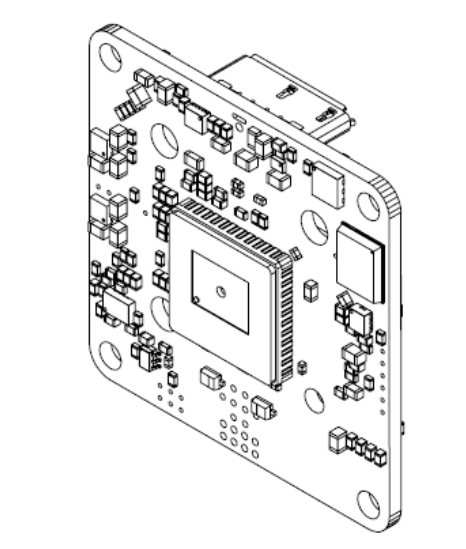
\includegraphics[width=0.25\textwidth]{images/camview.png}
	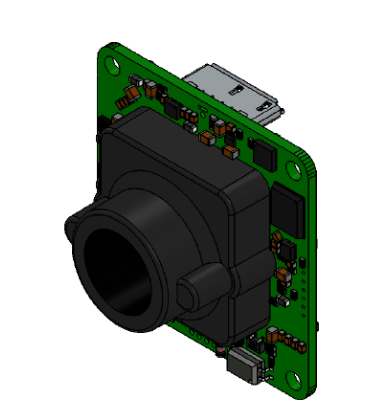
\includegraphics[width=0.25\textwidth]{images/camwlens.png}
	\caption[Camera uEye LE USB3]{On the left, the camera uEye LE's \acrshort{pcb}. On the right, the camera mounted with the lens holder.}
	\label{appendix:cha2:camview}
\end{figure}

\begin{figure}[ht]
	\centering
	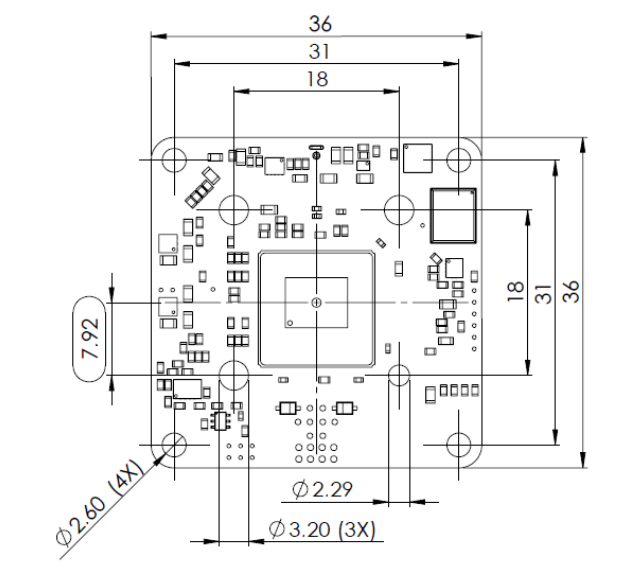
\includegraphics[width=0.35\textwidth]{images/camfronttview.png}
	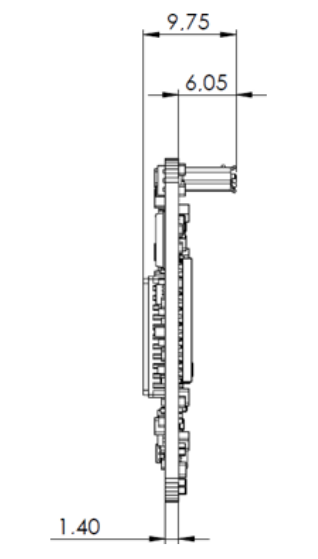
\includegraphics[width=0.25\textwidth]{images/camsideview.png}
	\caption[Camera uEye LE USB3's \acrshort{pcb}]{Camera uEye LE USB3's \acrshort{pcb} front view on the left and side view on the right. Measurements in millimeters.}
	\label{appendix:cha2:camsides}
\end{figure}

\begin{figure}[ht]
	\centering
	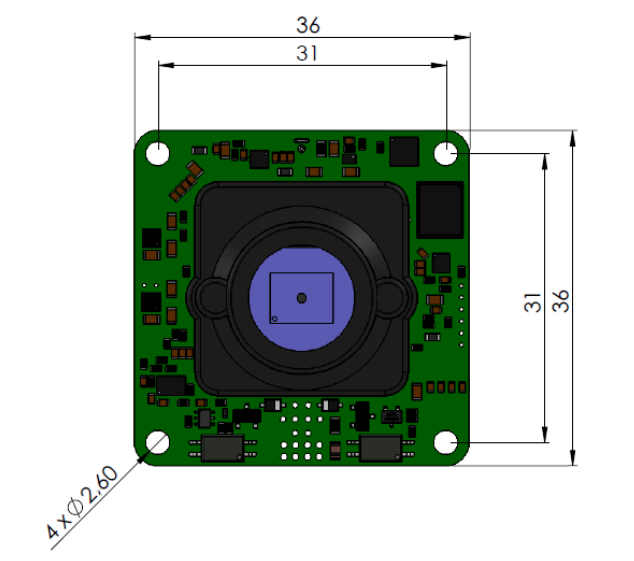
\includegraphics[width=0.35\textwidth]{images/camwlensfront.png}
	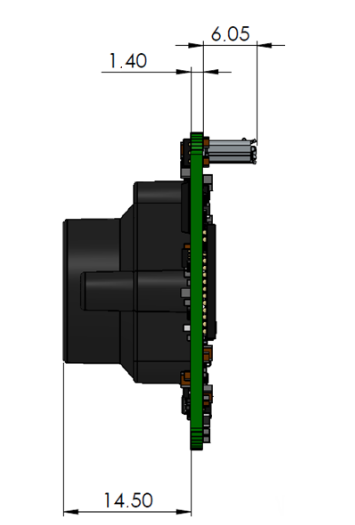
\includegraphics[width=0.25\textwidth]{images/camwlensside.png}
	\caption[Camera uEye LE USB3 with lens holder]{Camera uEye LE USB3 with lens holder from front view on the left and side view on the right. Measurements in millimeters.}
	\label{appendix:cha2:camwlens}
\end{figure}

\subsection{Lens}
\begin{figure}[ht]
	\centering
	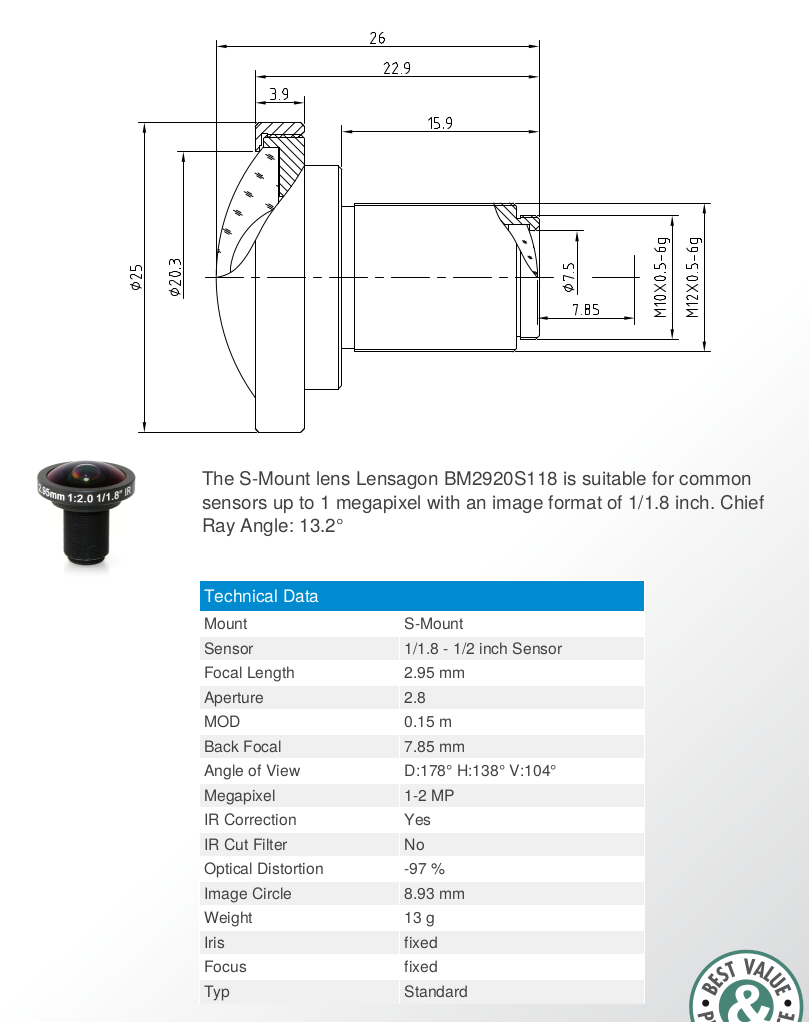
\includegraphics[width=0.9\textwidth]{images/lens.png}
	\caption[Lens BM2920S118 $2.95 \ mm$]{Datasheet from lens BM2920S118 with  $2.95 \ mm$ of focal length.}
	\label{appendix:cha2:lens}
\end{figure}

\subsection{Chessboard}
\label{appendix:cha2:chessboard}

\subsection{Calibration}

\section{\acrlong{imu}}
\label{appendix:cha2:imu}
\acrfull{lpmscu} 
The LpSensor library contains classes that allow a user to integrate LPMS devices into their own applications
\begin{figure}[ht]
	\centering
	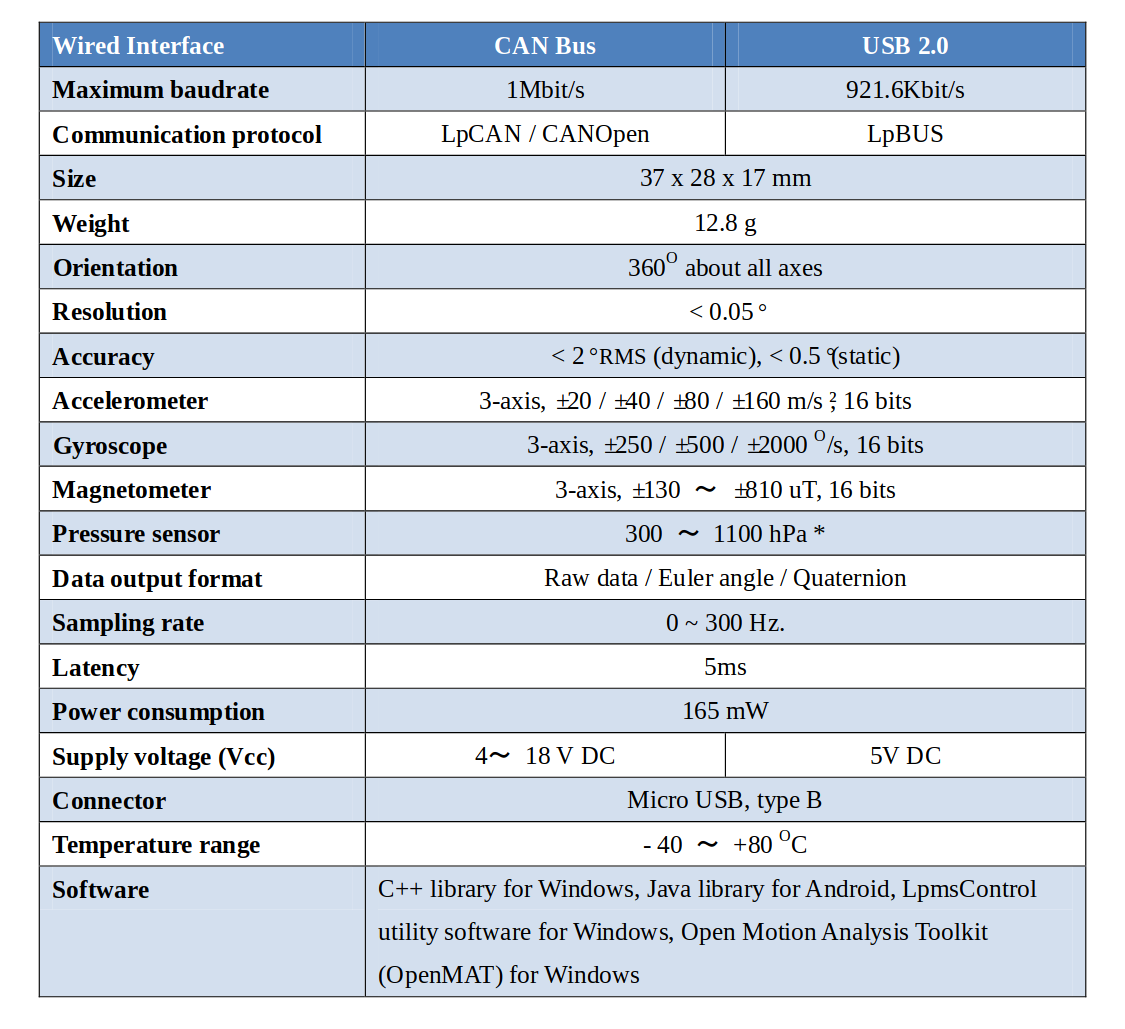
\includegraphics[width=\textwidth]{images/imuspecs.png}
	\caption[IMU specifications]{IMU specifications.}
	\label{appendix:cha2:eyescheme}
\end{figure}
